\chapter{The unscented Kalman filter}
\label{ch:ukf}

The EKF approximates the \emph{function} by a tangent plane and propagates
the Gaussian exactly through that approximation. The unscented Kalman
filter (UKF) does the opposite: it keeps the function exact and
approximates the \emph{distribution} by a handful of deterministically
chosen points, the \emph{sigma points}, then fits a Gaussian to where they
land. No Jacobian is needed, the mean is correct to one order higher, and,
as this chapter proves, the update automatically accounts for the
linearisation error that made the EKF over-confident.

\section{The unscented transform}

The problem is the one of \cref{prop:secondorder}: $X$ is Gaussian, $g$ is
non-linear, and we want the mean and the covariance of $g(X)$. The idea is
best seen in one dimension. Replace $\Normal(\mu,\sigma^2)$ by two points,
$\mu-\sigma$ and $\mu+\sigma$, each with weight $\tfrac12$. These two
points have the same mean and the same variance as the Gaussian. Apply $g$
to each, and take the mean and the variance of the two results. If $g$
bends, the two results are not symmetric about $g(\mu)$, and their average
moves away from it, as the true mean does.

In $n$ dimensions the same is done along $n$ directions, the columns of a
square root of the covariance, with a centre point added. The square root
used is the \emph{Cholesky factor} of $\Sigma$: the lower-triangular
matrix $L$ with $LL\T=\Sigma$, which exists and is unique (with a positive
diagonal) when $\Sigma$ is positive definite. Three parameters
tune the construction: $\alpha$ and $\kappa$ set how far from the mean the
points are placed, and $\beta$ adjusts the weight of the centre point in
the covariance.

\begin{definition}{Scaled sigma points}{sigma}
Let $\bmu\in\R^n$, $\Sigma\succ0$ with Cholesky factor $LL\T=\Sigma$
(columns $L_i$), and parameters $\alpha>0$, $\beta\ge0$, $\kappa$ with
$\lambda=\alpha^2(n+\kappa)-n>-n$. The $2n+1$ sigma points are
\[
  \chi_0=\bmu,\qquad\chi_{\pm i}=\bmu\pm\sqrt{n+\lambda}\,L_i,\quad
  i=1,\dots,n,
\]
with mean weights $W^{(m)}$ and covariance weights $W^{(c)}$:
\[
  W^{(m)}_0=\frac\lambda{n+\lambda},\quad
  W^{(c)}_0=W^{(m)}_0+1-\alpha^2+\beta,\quad
  W^{(m)}_{\pm i}=W^{(c)}_{\pm i}=\frac1{2(n+\lambda)}.
\]
The \emph{unscented transform} of $\Normal(\bmu,\Sigma)$ through $g$ is
\[
  \hat\y=\sum_jW^{(m)}_jg(\chi_j),\qquad
  P_y=\sum_jW^{(c)}_j\bigl(g(\chi_j)-\hat\y\bigr)
  \bigl(g(\chi_j)-\hat\y\bigr)\T .
\]
\end{definition}

\begin{figure}[ht]
\centering
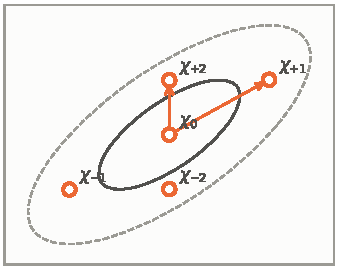
\includegraphics[width=0.45\linewidth]{figures/ch05_sigma_points.pdf}
\caption{The five sigma points of a two-dimensional Gaussian
($\alpha=1$, $\kappa=0$): the mean, and the mean $\pm\sqrt{n+\lambda}$
times each column of the Cholesky factor (arrows). Solid: the $1\sigma$
ellipse; dashed: $2\sigma$.}
\label{fig:sigmapoints}
\end{figure}

\Cref{fig:sigmapoints} shows the points for $n=2$. The columns $L_i$ of
the Cholesky factor play the role of $\sigma$ in one dimension: each is
one standard deviation of the Gaussian in one of $n$ independent
directions.

\begin{example}{The mean of a cosine}{utcos}
Take the example of \cref{fig:linearisation}: $\theta\sim\Normal(0.5,
0.8^2)$ and $g=\cos$. With the parameters used in this book ($\alpha=1$,
$\beta=2$, $\kappa=0$) and $n=1$, $\lambda=0$: the sigma points are $0.5$
and $0.5\pm0.8$, that is $-0.3$, $0.5$ and $1.3$, with mean weights
$\tfrac12$, $0$, $\tfrac12$. The unscented mean is
$\tfrac12(\cos(-0.3)+\cos1.3)=\tfrac12(0.955+0.267)=0.611$. The true mean
is $e^{-0.32}\cos0.5=0.637$, and linearisation gives $\cos0.5=0.878$.
The error falls from $0.878-0.637=0.241$ to $0.637-0.611=0.026$: two
evaluations of the function have removed nine tenths of it.
\end{example}

\begin{proposition}{Sigma points match the first two moments}{moments}
$\sum_jW^{(m)}_j=1$, $\sum_jW^{(m)}_j\chi_j=\bmu$ and
$\sum_jW^{(c)}_j(\chi_j-\bmu)(\chi_j-\bmu)\T=\Sigma$, and the same holds
with the mean weights $W^{(m)}_j$. All odd central moments of the weighted
points vanish.
\end{proposition}

\begin{proof}
Write $\vect\delta_j=\chi_j-\bmu$ for the offset of each point:
$\vect\delta_0=\vect0$ and $\vect\delta_{\pm i}=\pm\sqrt{n+\lambda}\,L_i$.

\emph{The weights add up to $1$.} The centre has the weight
$\lambda/(n+\lambda)$, and the $2n$ other points have
$1/(2(n+\lambda))$ each:
\[
  \sum_jW^{(m)}_j=\frac{\lambda}{n+\lambda}+2n\cdot\frac1{2(n+\lambda)}
  =\frac{\lambda+n}{n+\lambda}=1 .
\]

\emph{Odd moments vanish.} The points $\chi_{+i}$ and $\chi_{-i}$ have the
same weight and opposite offsets, so in any sum of an odd power of the
offsets (for instance $\sum_jW_j\vect\delta_j$, or
$\sum_jW_j\,\delta_{j,a}\delta_{j,b}\delta_{j,c}$ for three coordinates)
their two contributions cancel. The centre, with $\vect\delta_0=\vect0$,
contributes nothing to any central moment, whatever its weight.

\emph{The mean.} Then
$\sum_jW^{(m)}_j\chi_j=\bmu\sum_jW^{(m)}_j+\sum_jW^{(m)}_j\vect\delta_j
=\bmu\times1+\vect0=\bmu$.

\emph{The covariance.} The centre contributes nothing, and the two points
$\chi_{\pm i}$ have the same weight in both families of weights, so both
sums equal
\[
  \sum_{i=1}^n2\cdot\frac{1}{2(n+\lambda)}\,(n+\lambda)L_iL_i\T
  =\sum_{i=1}^nL_iL_i\T=LL\T=\Sigma,
\]
because $\vect\delta_{\pm i}\vect\delta_{\pm i}\T=(n+\lambda)L_iL_i\T$,
and a matrix times its transpose is the sum of the products of its
columns, $LL\T=\sum_iL_iL_i\T$.
\end{proof}

\begin{theorem}{The unscented mean is exact up to third order}{utorder}
Let $X\sim\Normal(\bmu,\Sigma)$. If every component of $g$ is a
polynomial of degree at most $3$, then $\hat\y=\E[g(X)]$. For a smooth
$g$ with bounded fourth derivatives, $\hat\y-\E[g(X)]=O(\norm\Sigma^2)$,
whereas the linearised mean $g(\bmu)$ has an error of order
$\norm\Sigma$ (\cref{prop:secondorder}).
\end{theorem}

\begin{proof}
Compare, term by term, the Taylor expansion of $g_i$ around $\bmu$
averaged in two ways: over $X$ (the true mean) and over the weighted
sigma points (the unscented mean). With $\vect\delta$ the offset from
$\bmu$ ($\vect e=X-\bmu$ for $X$, $\vect\delta_j=\chi_j-\bmu$ for the
points),
\[
  g_i(\bmu+\vect\delta)=g_i(\bmu)+\nabla g_i\T\vect\delta
  +\tfrac12\vect\delta\T\nabla^2g_i\,\vect\delta
  +\tfrac16D^3g_i[\vect\delta,\vect\delta,\vect\delta]+\rho(\vect\delta).
\]
\begin{itemize}[nosep]
  \item \emph{Constant term.} $g_i(\bmu)$ on both sides, since both sets of
        weights add up to $1$.
  \item \emph{First- and third-order terms.} Zero on both sides: for $X$
        because the odd moments of a centred Gaussian are zero (proof of
        \cref{prop:secondorder}), for the sigma points by
        \cref{prop:moments}.
  \item \emph{Second-order term.} $\tfrac12\tr(\nabla^2g_i\Sigma)$ on both
        sides. For $X$ this is the proof of \cref{prop:secondorder}. For
        the points, with the trace identity used there and
        \cref{prop:moments},
        \[
          \sum_jW^{(m)}_j\tfrac12\vect\delta_j\T\nabla^2g_i\vect\delta_j
          =\tfrac12\tr\Bigl(\nabla^2g_i\sum_jW^{(m)}_j\vect\delta_j
          \vect\delta_j\T\Bigr)=\tfrac12\tr(\nabla^2g_i\Sigma).
        \]
\end{itemize}
For a polynomial of degree at most $3$ there is no remainder $\rho$, so
the two means coincide. Otherwise each side
keeps a fourth-order remainder: $O(\norm\Sigma^2)$ for $X$ (proof of
\cref{prop:secondorder}), and at most $C\norm{\vect\delta_j}^4\le
C(n+\lambda)^2\norm\Sigma^2$ at each sigma point, since
$\norm{L_i}^2\le\norm\Sigma$. The two means therefore differ by
$O(\norm\Sigma^2)$.
\end{proof}

\begin{inwords}
Seven points (in three dimensions) are enough to capture the curvature
term that the EKF misses. The UKF does not differentiate anything: it
simply evaluates the model at well-placed points and lets the model's own
curvature show up in the results.
\end{inwords}

The covariance $P_y$ is correct to first order, like the EKF's, and
captures part of the higher-order terms; $\beta$ adds information about
the fourth moment. (These statements are not proved here; see Julier and
Uhlmann, and Wan and van der Merwe, in the references. The next example
can be checked by hand.) For $y=x^2$ with $x\sim\Normal(\mu,\sigma^2)$, the
choice $\alpha=1$, $\beta=2$, $\kappa=0$ gives both the mean
$\mu^2+\sigma^2$ and the variance $4\mu^2\sigma^2+2\sigma^4$
\emph{exactly}, where linearisation gives $\mu^2$ and $4\mu^2\sigma^2$
(Exercise~\ref{ex:square}).

\paragraph{Choosing the parameters.} The original choice $\lambda=3-n$
($\alpha=1$, $\kappa=3-n$, $\beta=0$) matches the Gaussian kurtosis (the
fourth moment, $3\sigma^4$) along each axis (Exercise~\ref{ex:kurtosis}), but makes the centre weight
$W_0=(3-n)/3$ \emph{negative} as soon as $n>3$. A negative weight in a
covariance can produce an indefinite $P_y$ (Exercise~\ref{ex:negative}),
after which the next Cholesky factorisation fails. This book uses
$\alpha=1$, $\beta=2$, $\kappa=0$, so that $\lambda=0$, $W^{(m)}_0=0$ and
$W^{(c)}_0=2$: every covariance weight is non-negative.

\Cref{fig:utarc} replays the arc of \cref{fig:arc} with the unscented
transform. The exact mean is $(40e^{-0.32},0)=(29.05,0)$ (Exercise
\ref{ex:ecos}); the UKF's mean is $0.08$ units from it, the EKF's about
$11$. The UKF's ellipse covers the arc, but it is too wide along the
direction of travel (standard deviation $21.8$ against $13.4$) and
slightly too narrow across it ($22.7$ against $24.1$). Notebook~04
computes these exact values from Exercises~\ref{ex:ecos}
and~\ref{ex:cosvar} and compares. Neither can represent the arc itself: both summarise
it by a Gaussian.

\begin{figure}[ht]
\centering
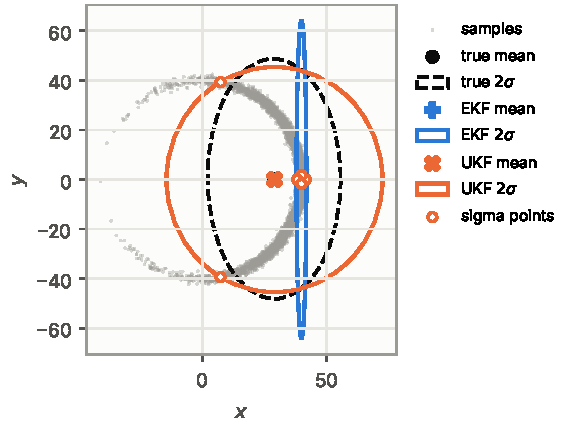
\includegraphics{figures/ch05_arc.pdf}
\caption{The arc of \cref{fig:arc}: forty units driven with a $45^\circ$ heading
uncertainty. Grey: $5\,000$ samples of the true distribution, with its
mean and $2\sigma$ ellipse (dashed). Blue: the EKF's prediction. Orange:
the unscented transform, with its seven transformed sigma points.}
\label{fig:utarc}
\end{figure}

\section{The filter}

The filter uses the unscented transform twice per cycle: through the
motion model $f$ for the prediction, and through the sensor model $h$ for
the update.

\paragraph{Non-additive noise.} The control noise acts inside the motion
model, $f(\x,\uu+\bepsilon)$: the turn error is applied before the robot
drives. It enters $f$ non-linearly and cannot simply be added as a $Q$.
The standard remedy is to \emph{augment} the state with the noise,
\[
  \x^a=\begin{pmatrix}\x\\\bepsilon\end{pmatrix}\sim
  \Normal\left(\begin{pmatrix}\hx\\\vect0\end{pmatrix},
  \begin{pmatrix}P&0\\0&M\end{pmatrix}\right),\qquad n_a=3+2=5,
\]
draw $2n_a+1=11$ sigma points and push each through
$f(\x,\uu+\bepsilon)$. Each augmented sigma point $\chi^a_j$ has five
components: the first three, written $\chi^x_j$, are a pose, and the last
two, written $\chi^\varepsilon_j$, are a control noise. The measurement
noise is additive and does not need augmentation.

\paragraph{The update.} The prediction gives a new Gaussian
$\Normal(\bx,\bar P)$, so new sigma points $\chi_j$ are drawn from it,
seven of them. Pushing them through the sensor model, $Z_j=h(\chi_j)$,
gives sigma-point estimates of three quantities: the predicted measurement
$\hat\z$, the covariance $S$ of the measurement (to which the sensor noise
$R$ is added), and the cross-covariance $P_{xz}=\Cov(\x,\z)$ between the
pose and the measurement. The update is then \cref{thm:conditioning},
applied as if $(\x,\z)$ were jointly Gaussian with these moments: the gain
is $\Sigma_{xy}\Sigma_{yy}^{-1}=P_{xz}S^{-1}$, and the covariance decreases
by $\Sigma_{xy}\Sigma_{yy}^{-1}\Sigma_{yx}=P_{xz}S^{-1}P_{xz}\T
=(P_{xz}S^{-1})S(P_{xz}S^{-1})\T=KSK\T$.

\begin{definition}{Unscented Kalman filter}{ukf}
\emph{Predict}: sigma points $\chi^a_j$ of the augmented Gaussian;
$\chi'_j=f(\chi^x_j,\uu+\chi^\varepsilon_j)$; $(\bx,\bar P)$ is the
unscented transform of these points.

\emph{Update}: fresh sigma points $\chi_j$ of $\Normal(\bx,\bar P)$;
$Z_j=h(\chi_j)$;
\begin{gather*}
  \hat\z=\sum_jW^{(m)}_jZ_j,\qquad
  S=\sum_jW^{(c)}_j(Z_j-\hat\z)(Z_j-\hat\z)\T+R,\\
  P_{xz}=\sum_jW^{(c)}_j(\chi_j-\bx)(Z_j-\hat\z)\T,\qquad
  K=P_{xz}S^{-1},\\
  \hx=\bx+K(\z-\hat\z),\qquad P=\bar P-KSK\T .
\end{gather*}
Heading and bearing components are averaged on the circle and every
residual is wrapped (\cref{sec:ukf-angles}).
\end{definition}

For a linear $h(\x)=H\x$ these are $P_{xz}=\bar PH\T$ and
$S=H\bar PH\T+R$: by \cref{prop:moments}, $\hat\z=H\bx$, so
$Z_j-\hat\z=H(\chi_j-\bx)$, and the sums become
$\bigl(\sum_jW^{(c)}_j(\chi_j-\bx)(\chi_j-\bx)\T\bigr)H\T=\bar PH\T$ and
$H\bar PH\T$. The update is then exactly the Kalman update of
\cref{thm:kf}. In general it is
that update with $\bar PH\T$ and $H\bar PH\T+R$ replaced by their
sigma-point estimates. What does that replacement do?

\Cref{fig:regression} shows it in one dimension. The EKF replaces $h$ by
its tangent at the mean. The UKF never computes a slope, but its update
behaves as if $h$ had been replaced by another straight line: the one that
fits the values of $h$ at the sigma points best, in the least-squares
sense: among the lines through $(\bx,\hat\z)$, the one with the slope $A$
that minimises $\sum_jW^{(c)}_j\norm{Z_j-\hat\z-A(\chi_j-\bx)}^2$. This is a \emph{regression} line, and its slope is
$\Cov(\z,\x)\Cov(\x)^{-1}$, the regression coefficient already met in
\cref{thm:conditioning}; here it is $\tilde H=P_{xz}\T\bar P^{-1}$. To see
it, write $\vect\delta_j=\chi_j-\bx$. With non-negative weights the sum
is a convex quadratic in $A$, so its minimum is where its derivative with
respect to $A$ vanishes:
\[
  \sum_jW^{(c)}_j\bigl(Z_j-\hat\z-A\vect\delta_j\bigr)\vect\delta_j\T=0,
  \qquad\text{that is}\qquad
  \underbrace{\sum_jW^{(c)}_j(Z_j-\hat\z)\vect\delta_j\T}_{P_{xz}\T}
  =A\underbrace{\sum_jW^{(c)}_j\vect\delta_j\vect\delta_j\T}_{\bar P},
\]
the second sum being $\bar P$ by \cref{prop:moments}. So
$A=P_{xz}\T\bar P^{-1}$. Because
$h$ is curved, the sigma points do not lie exactly on that line. Their
scatter around it is what a straight line cannot explain, and the UKF
counts it as extra measurement noise. The next theorem states this
precisely; ``statistically linearised'' is the usual name for a slope
obtained by regression instead of differentiation.

\begin{figure}[ht]
\centering
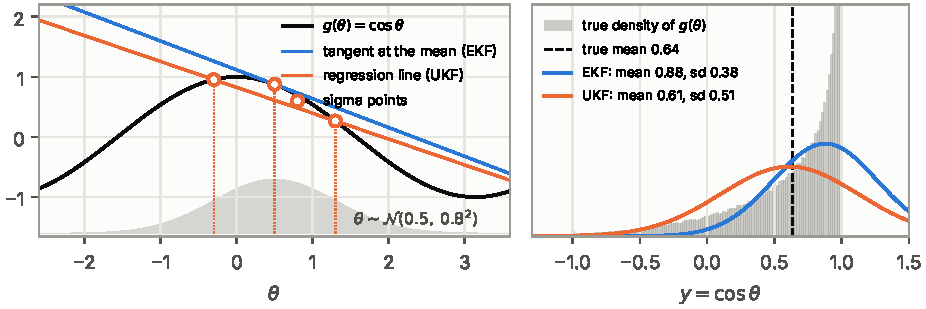
\includegraphics[width=\linewidth]{figures/ch05_regression.pdf}
\caption{The example of \cref{fig:linearisation}, with the unscented transform
added: an angle $\theta\sim\Normal(0.5,0.8^2)$ (grey density, left) is
passed through $\cos$. The UKF evaluates $\cos$ at three sigma points and fits a
regression line through them (slope $\tilde H=-0.43$; the tangent's is
$-0.48$). The two outer points lie on that line; the centre point is off
it by $0.27$, and the weighted scatter, $\Omega=0.14$, is added to the
output variance. The UKF's mean ($0.61$) is
close to the true mean ($0.64$), and its spread covers the true
distribution.}
\label{fig:regression}
\end{figure}

\begin{theorem}{The UKF update is a Kalman update with an inflated $R$}{slr}
Assume all $W^{(c)}_j\ge0$. Define the \emph{statistically linearised}
measurement matrix $\tilde H=P_{xz}\T\bar P^{-1}$ and the residuals
$\vect\zeta_j=Z_j-\hat\z-\tilde H(\chi_j-\bx)$. Then
\[
  P_{xz}=\bar P\tilde H\T,\qquad
  S=\tilde H\bar P\tilde H\T+R+\Omega,\qquad
  \Omega=\sum_jW^{(c)}_j\vect\zeta_j\vect\zeta_j\T\succeq0,
\]
so the UKF update is the Kalman update for the affine model
$\z=\hat\z+\tilde H(\x-\bx)+\vv'$ with noise covariance
$R+\Omega\succeq R$.
\end{theorem}

\begin{proof}
\emph{The cross-covariance.} From $\tilde H=P_{xz}\T\bar P^{-1}$,
$\tilde H\T=\bar P^{-1}P_{xz}$ ($\bar P$ is symmetric), so
$\bar P\tilde H\T=P_{xz}$.

\emph{The residuals are uncorrelated with the offsets.} Write
$\vect\delta_j=\chi_j-\bx$, so that
$Z_j-\hat\z=\tilde H\vect\delta_j+\vect\zeta_j$ by the definition of
$\vect\zeta_j$. Then
\[
  \sum_jW^{(c)}_j\vect\zeta_j\vect\delta_j\T
  =\sum_jW^{(c)}_j(Z_j-\hat\z)\vect\delta_j\T
   -\tilde H\sum_jW^{(c)}_j\vect\delta_j\vect\delta_j\T
  =P_{xz}\T-\tilde H\bar P=0 ,
\]
using \cref{prop:moments} for the second sum and the first step for the
last equality.

\emph{The innovation covariance.} By the definition of $S$ and the same
decomposition,
\begin{align*}
  S-R&=\sum_jW^{(c)}_j(\tilde H\vect\delta_j+\vect\zeta_j)
       (\tilde H\vect\delta_j+\vect\zeta_j)\T\\
  &=\tilde H\Bigl(\sum_jW^{(c)}_j\vect\delta_j\vect\delta_j\T\Bigr)\tilde H\T
   +\tilde H\sum_jW^{(c)}_j\vect\delta_j\vect\zeta_j\T
   +\sum_jW^{(c)}_j\vect\zeta_j\vect\delta_j\T\tilde H\T
   +\sum_jW^{(c)}_j\vect\zeta_j\vect\zeta_j\T\\
  &=\tilde H\bar P\tilde H\T+0+0+\Omega .
\end{align*}
$\Omega$ is a combination, with non-negative weights, of the positive
semi-definite matrices $\vect\zeta_j\vect\zeta_j\T$, hence positive
semi-definite.

\emph{The equivalent Kalman update.} The affine model of the statement
has the cross-covariance $\Cov(\x,\tilde H\x+\vv')=\bar P\tilde H\T=
P_{xz}$ and the innovation covariance $\tilde H\bar P\tilde H\T+R+\Omega=
S$. Its Kalman gain $P_{xz}S^{-1}$ and its updated covariance
$\bar P-KSK\T$ are therefore those of the UKF.
\end{proof}

\begin{inwords}
The UKF fits the best straight line to $h$ over the sigma points (a
weighted least-squares regression, not a tangent at one point), and
whatever that line cannot explain is added to the measurement noise. When
$h$ is nearly linear over the uncertainty, $\Omega\approx0$ and the UKF is
the EKF. When it is not, the UKF trusts the measurement less, exactly
where the EKF trusted it too much. This is why it is much less
over-confident after an uncertain start (\cref{fig:ukftransient}).
\end{inwords}


\section{Angles in the UKF}
\label{sec:ukf-angles}

Two components of the state and of the measurement are angles: the
heading, and the bearing of each landmark. They need care at two places.

\emph{Means.} The unscented transform averages the sigma points with the
weights $W^{(m)}_j$. For an angle component the plain average can point
the wrong way when the points straddle the cut at $\pm\pi$, so these
components are averaged with the circular mean of \cref{sec:circular}
instead (with the weights of this book, every $W^{(m)}_j$ is
non-negative).

\emph{Differences.} The same care is needed in the covariances. $P_y$,
$P_{xz}$ and the innovation are built from differences between an angle
and a mean angle, $\theta_j-\bar\theta$, and such a difference can be off
by $\pm2\pi$ (\cref{lem:wrap}). With $\theta_j=3.1$ and
$\bar\theta=-3.13$, the plain difference is $6.23$ where the rotation is
$-0.05$, and its square, $38.8$ instead of $0.0028$, would make the
covariance absurd. So every difference of angles is wrapped before it
enters a covariance or an innovation.

\section{Where the UKF earns its keep}

With four landmarks in view and a good start, the UKF and the EKF are
indistinguishable on the standard run (RMSE $0.99$ against $1.01$,
notebook~04): the models are nearly linear over the small uncertainty.
The UKF costs about 50\% more per step ($0.15$ against $0.10$\,ms in the
comparison of \cref{ch:choosing}, notebook~06; the exact figures depend
on the machine), for
$11+7$ model evaluations and two Cholesky factorisations instead of two
Jacobians.

After the uncertain start of \cref{fig:ekftransient}, however, the two
filters differ sharply (\cref{fig:ukftransient}). With the same runs and
the same initial estimates, the UKF's average NEES is $12$ after the first
update, $3.0$ after five and $2.9$ after twenty (EKF: $297$, $63$, $6.5$;
notebook~04 prints both), and its error drops slightly faster.

\begin{figure}[ht]
\centering
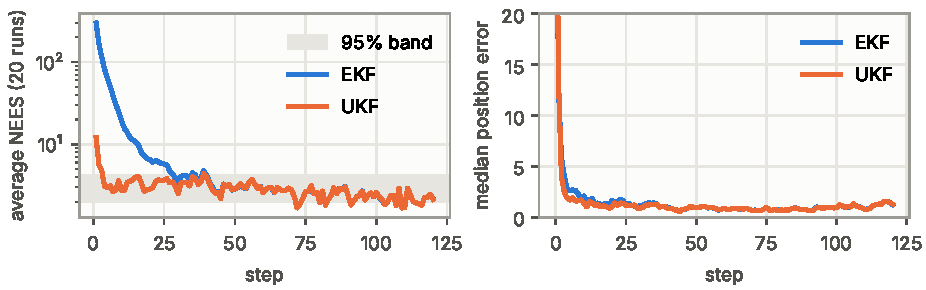
\includegraphics[width=\linewidth]{figures/ch05_transient.pdf}
\caption{The uncertain start of \cref{fig:ekftransient}, with both filters on the
same $20$ runs: the initial estimate is drawn from $\Normal(\x_0,P_0)$
with $\sigma_{xy}=30$ and $\sigma_\theta=0.8$. Left: average NEES (log
scale) and its $95\%$ band for $n=3$. Right: median position error. The UKF is within the band after a few
updates; the EKF is over-confident by up to two orders of magnitude.}
\label{fig:ukftransient}
\end{figure}

\begin{practice}[\nb{04\_unscented\_kalman\_filter.ipynb}, \code{ukf.py}]
\code{merwe\_weights}, \code{sigma\_points} and \code{unscented\_transform}
implement \cref{def:sigma}; \code{pose\_mean}, \code{meas\_mean} and the
residual functions handle the angles. \code{UKF} augments the state with
the control noise for the prediction and regenerates seven sigma points
for each update. A unit test checks that the transform is exact for
linear maps for several $(\alpha,\kappa)$, the cheapest possible guard
against the classic sigma-point bugs (a missing point, a spread of
$n+\lambda$ instead of $\sqrt{n+\lambda}$). The notebook reproduces
\cref{fig:utarc,fig:ukftransient}.
\end{practice}

\begin{mower}
The UKF is attractive whenever the Jacobians are tedious or error-prone:
with a camera model, an IMU on a chassis that pitches and rolls, or GNSS
antenna lever arms. Its cost grows with the number of sigma points,
linearly in the state dimension, and each point needs one evaluation of
the models; for the few-dimensional state of a mower this is negligible.
\end{mower}

\section*{What to remember from this chapter}
\addcontentsline{toc}{section}{What to remember}

\begin{enumerate}[nosep]
  \item The unscented transform replaces a Gaussian by $2n+1$ weighted
    points with the same mean and covariance, pushes them through the
    exact non-linear function, and fits a Gaussian to the results. No
    Jacobian is needed.
  \item Its mean is exact for polynomials up to degree $3$: it captures
    the curvature term that the EKF misses.
  \item The UKF is a Kalman filter in which the predicted mean and
    covariance, the innovation covariance $S$ and the cross-covariance
    $P_{xz}$ are computed from sigma points. The control noise is handled
    by augmenting the state.
  \item Its update is a Kalman update with the regression slope $\tilde H$
    and an inflated noise $R+\Omega$: what a straight line cannot explain
    is counted as noise. This keeps the UKF consistent where the EKF is
    over-confident.
  \item Angles need care: headings and bearings are averaged with the
    circular mean, and every residual is wrapped.
  \item The covariance weights must be non-negative, or the computed
    covariances may fail to be positive semi-definite; the parameters
    $\alpha=1$, $\beta=2$, $\kappa=0$ guarantee it.
\end{enumerate}

\FloatBarrier
\section*{Exercises}
\addcontentsline{toc}{section}{Exercises}

\begin{enumerate}[label=\textbf{5.\arabic*},ref=5.\arabic*]
\item\label{ex:square} Let $x\sim\Normal(\mu,\sigma^2)$ and $y=x^2$.
  Compute the unscented mean and variance of $y$ for $n=1$ and general
  $\lambda$, $W^{(c)}_0$. Show that they are exact if and only if
  $W^{(c)}_0+(n+\lambda-1)^2/(n+\lambda)=2$, and check the choice of this
  book.
\item\label{ex:kurtosis} For $n=1$, show that the sigma points with
  $n+\kappa=3$ (and $\alpha=1$) reproduce the fourth moment $3\sigma^4$ of
  a Gaussian.
\item\label{ex:negative} Take $\lambda=3-n$ with $n=5$ and $\beta=0$, so
  $W^{(c)}_0=W^{(m)}_0=w<0$. Let $g$ take one value $a$ at $\chi_0$ and
  another value $b$ at every other sigma point. Show that the unscented
  variance is $(a-b)^2w(1-w)<0$.
\end{enumerate}

\subsection*{Solutions}

\solution{5.1} \emph{The sigma points.} For $n=1$, write $c^2=n+\lambda
=1+\lambda$. By \cref{def:sigma} the points are $\mu$ and $\mu\pm c\sigma$;
the outer points have the weight $1/(2c^2)$ each, and the centre has the
mean weight $W^{(m)}_0=1-2\cdot\frac1{2c^2}=1-1/c^2$ and the covariance
weight $W^{(c)}_0$. The values of $y=x^2$ are
\[
  y_0=\mu^2,\qquad y_\pm=(\mu\pm c\sigma)^2=\mu^2\pm2\mu c\sigma+c^2\sigma^2 .
\]

\emph{The unscented mean.} In the sum $y_++y_-$ the terms $\pm2\mu c\sigma$
cancel:
\[
  \hat y=W^{(m)}_0\mu^2+\frac1{2c^2}\bigl(2\mu^2+2c^2\sigma^2\bigr)
  =\Bigl(W^{(m)}_0+\frac1{c^2}\Bigr)\mu^2+\sigma^2=\mu^2+\sigma^2 ,
\]
exact for any parameters, as \cref{thm:utorder} says for a polynomial of
degree $2$.

\emph{The unscented variance.} The deviations from $\hat y$ are
$y_0-\hat y=-\sigma^2$ at the centre and
$y_\pm-\hat y=\pm2\mu c\sigma+(c^2-1)\sigma^2$ at the others. Squaring,
\[
  (y_\pm-\hat y)^2=4\mu^2c^2\sigma^2\pm4\mu c\sigma(c^2-1)\sigma^2
  +(c^2-1)^2\sigma^4 ,
\]
and in the sum of the two the middle terms cancel. With the weights,
\[
  P_y=W^{(c)}_0\sigma^4+\frac1{2c^2}\cdot2\bigl(4\mu^2c^2\sigma^2
  +(c^2-1)^2\sigma^4\bigr)
  =4\mu^2\sigma^2+\Bigl(W^{(c)}_0+\frac{(c^2-1)^2}{c^2}\Bigr)\sigma^4.
\]

\emph{The true variance.} Write $x=\mu+e$ with $e\sim\Normal(0,\sigma^2)$.
Then $x^2=\mu^2+2\mu e+e^2$ and $\E[x^2]=\mu^2+\sigma^2$, so
$x^2-\E[x^2]=2\mu e+(e^2-\sigma^2)$, and
\begin{align*}
  \Var(x^2)&=\E\bigl[(2\mu e+e^2-\sigma^2)^2\bigr]
  =4\mu^2\E[e^2]+4\mu\,\E\bigl[e(e^2-\sigma^2)\bigr]
   +\E\bigl[(e^2-\sigma^2)^2\bigr]\\
  &=4\mu^2\sigma^2+0+\bigl(\E[e^4]-2\sigma^2\E[e^2]+\sigma^4\bigr)
  =4\mu^2\sigma^2+(3\sigma^4-2\sigma^4+\sigma^4)
  =4\mu^2\sigma^2+2\sigma^4,
\end{align*}
using $\E[e^3]=\E[e]=0$ (symmetry) and $\E[e^4]=3\sigma^4$
(\cref{ex:gaussmoments}).

\emph{When they agree.} The $\mu^2$ terms always agree, and the
$\sigma^4$ terms agree exactly when $W^{(c)}_0+(c^2-1)^2/c^2=2$. With the
choice of this book, $\alpha=1$, $\beta=2$, $\kappa=0$: $\lambda=0$, so
$c^2=1$, $W^{(m)}_0=0$ and $W^{(c)}_0=0+1-1+2=2$, and
$2+0=2$: exact. (With $\kappa=2$ and $\beta=2$, $c^2=3$ and
$W^{(c)}_0=\frac23+2=\frac83$, so $\frac83+\frac43=4$: the quartic term
is $4\sigma^4$, twice too much.)

\solution{5.2} With $\alpha=1$, $\lambda=\alpha^2(n+\kappa)-n=\kappa$, so
$n+\lambda=n+\kappa=3$, and the outer points are
$\mu\pm\sqrt{n+\lambda}\,\sigma=\mu\pm\sqrt3\,\sigma$. They have the weight
$\frac1{2(n+\lambda)}=\frac16$ each, and the centre adds nothing to a
central moment, so
\[
  \sum_jW_j(\chi_j-\mu)^4=2\cdot\frac16\cdot(\sqrt3\,\sigma)^4
  =\frac13\cdot9\sigma^4=3\sigma^4,
\]
the fourth moment of $\Normal(\mu,\sigma^2)$ (\cref{ex:gaussmoments}).
For larger $n$ the same holds along each axis of the Cholesky factor, but
the cross moments, such as $\E[e_1^2e_2^2]$, do not match.

\solution{5.3} \emph{The weight.} With $n=5$ and $\lambda=3-n=-2$, the
centre has the weight $w=\lambda/(n+\lambda)=-2/3$, and since $\beta=0$
and $\alpha=1$, $W^{(c)}_0=w+1-1+0=w$. The other ten points share the
weight $1-w$.

\emph{The mean.} $\hat y=wa+(1-w)b$.

\emph{The deviations.} At the centre, $a-\hat y=(1-w)a-(1-w)b
=(1-w)(a-b)$; at the other points, $b-\hat y=-w(a-b)$.

\emph{The variance.}
\[
  P_y=w\bigl((1-w)(a-b)\bigr)^2+(1-w)\bigl(w(a-b)\bigr)^2
  =(a-b)^2w(1-w)\bigl[(1-w)+w\bigr]=(a-b)^2w(1-w),
\]
which is negative when $w<0$. For $n=5$, $w(1-w)=-\frac23\cdot\frac53
=-\frac{10}9$, and $P_y=-\frac{10}9(a-b)^2$: a ``variance'' that is
negative.
